\chapter{Signal flow diagrams}
\section{Introduction}

The remit of this paper is the development of a sound and fully complete
equational theory of linear time-invariant (LTI) dynamical systems.  This theory
is \emph{graphical}, with its terms---modelling the LTI
systems themselves---best represented as diagrams closely resembling the signal
flow graphs of Shannon~\cite{Sh}.  

To acquaint ourselves with signal flow graphs, we begin with the example below,
rendered in traditional, directed notation.
\begin{equation}\label{eq:examplesfg}
  \begin{aligned}
\lower11pt\hbox{$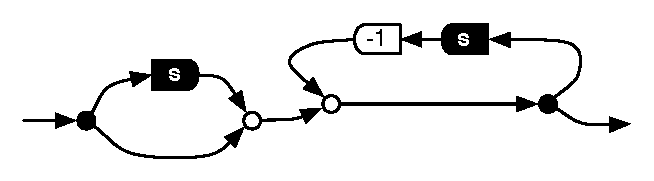
\includegraphics[height=1.5cm]{pics/examplesfg.pdf}$}
\end{aligned}
\end{equation}
This system takes, as input on the left, a stream of values from a field $\k$,
e.g.\ the rational numbers, and on the right outputs a processed stream of
values. The white circles are adders, the black circles are duplicators, the
$s$ gates are 1-step delays and the $-1$ gate is an instance of an amplifier
that outputs $-1$ times its input. Processing is done synchronously according to
a global clock. 

For instance, assume that at time $0$ the left $s$ gate `stores' the value $1$
and the right $s$ gate stores $2$. Given an input of $-1$, the flow graph first
adds the left stored value $1$, and then adds $-1 \times 2$, for an output of
$-2$. Immediately after this time step the $s$ gates, acting as delays, now
store $-1$ and $-2$ respectively, and we repeat the process with the next input.
Thus from this time $0$ an input stream of $-1,1,-1,1\dots$ results in an output
stream of $-2,2,-2,2,\dots$.

We can express \eqref{eq:examplesfg} as a string diagram, a notation for the
arrows of monoidal categories made popular by Joyal and Street \cite{JS}, by
forgetting the directionality of wires and composing the following basic
building blocks using the operations of monoidal categories.
\begin{multline*}
\copygen \mathrel{;} 
\!\!\!\!\!\!\!
\begin{array}{c} \delaygen \\ \oplus \\ \id \end{array} 
\!\!\!\!\!\!\!\mathrel{;}\!\! \addgen
\mathrel{;} \!\!\!\!\!\!\! \begin{array}{c} \discardopgen \\ \oplus \\ \id \end{array} 
\!\!\!\!\!
\mathrel{;} 
\!\!\!\!\!
 \begin{array}{c} \copygen \\ \oplus \\ \id \end{array} 
\!\!\!\!\!
\mathrel{;}
\\
\!\!\!\!\! 
 \begin{array}{c} \minonegen \\ \oplus \\ \id \end{array} 
\!\!\!\!\! 
 \mathrel{;}
\!\!\!\!\! 
 \begin{array}{c} \delayopgen \\ \oplus \\ \id \end{array} 
 \!\!\!\!\! 
 \mathrel{;}
\!\!\!\!\! 
 \begin{array}{c} \id \\ \oplus \\ \copygen \end{array} 
  \!\!\!\!\! 
 \mathrel{;}
\!\!\!\!\! 
 \begin{array}{c} \copyopgen \\ \oplus \\ \id \end{array} 
 \!\!\!\!\! 
 \mathrel{;}
\!\!\!\!\! 
 \begin{array}{c} \discardgen \\ \oplus \\ \id \end{array} 
\end{multline*}
The building blocks come from the signature of an algebraic theory---a
\emph{symmetric monoidal theory} to be exact. The terms of this theory comprise
the morphisms of a \emph{prop}, a symmetric monoidal category in which the
objects are the natural numbers. With an operational semantics suggested by the
above example, the terms can also be considered as a process
algebra for signal flow graphs. The idea of understanding complex 
systems by ``tearing'' them into more basic components, ``zooming'' to
understand their individual behaviour and ``linking'' to obtain a composite
system is at the core of the behavioural approach in control, originated by
Willems~\cite{Wi3}. The algebra of symmetric monoidal categories thus seems a
good fit for a formal account of these compositional principles.

This paper is the first to make this link between monoidal categories and the
behavioural approach to control explicit. Moreover, it is the first to endow
signal flow graphs with their standard systems theoretic semantics in which the
registers---the `$s$' gates---are permitted to hold \emph{arbitrary} values at
the beginning of a computation (in previous work~\cite{BSZ1,BSZ3} they were
initialised with $0$).  This extended notion of behaviour is not merely a
theoretical curiosity: it gives the class of \emph{complete LTI discrete
dynamical systems}~\cite{Wi3}, which is practically the lingua franca of control
theory. The interest of systems theorists is due to practical considerations:
physical systems seldom evolve from zero initial conditions.

Technically, the semantics of diagrams are sets of \emph{biinfinite}
streams: those sequences of elements of $\k$ that are infinite in the past
\emph{as well} as in the future---that is, elements of $\k^\z$.  Starting with
the operational description, one obtains a biinfinite trajectory by executing
circuits forwards and backwards in time, for some initialisation of the
registers. The dynamical system defined by a signal flow diagram is the set of
trajectories obtained by considering all possible executions from all possible initialisations.

An equational theory also requires equations between the terms. We obtain the
equations in two steps. First, we show there is a full, but not faithful,
morphism from the prop $\cospan\mat\pk$ of cospans of matrices over the ring
$\pk$ to the prop $\ltids$ of complete LTI discrete dynamical systems.
Using the presentation of $\cospan\mat\pk$ in~\cite{BSZ2,Za}, the result is a
sound, but not complete, proof system. The second ingredient is restricting our
attention from cospans to jointly-epic cospans, or \emph{corelations}. This
gives a faithful morphism, allowing us to present the prop of corelations as a
symmetric monoidal theory, and hence giving a sound and complete proof system for
reasoning about LTIs (Theorem \ref{thm.main}).

The advantages of the string diagram calculus over the traditional matrix
calculus are manifold. The operational semantics make the notation intuitive, as
does the compositional aspect: it is cumbersome to describe connection of
systems using matrices, whereas with string diagrams you just connect the right
terminals. Moreover, the calculus unifies the variety of distinct methods for representing
LTI systems with matrix equations---built from kernel and image
representations~\cite{Wi,Wi3}---into a single framework, heading off
possibilities for ambiguity and confusion.

We hope, however, the greatest advantage will be the way these properties can be
leveraged in analysis of controllability. In Theorem \ref{cor.spanreps}, we
show that in our setting controllability has an elegant structural
characterisation.  Compositionality pays off here, with our proof system giving
a new technique for reasoning about control of compound systems (Prop.
\ref{prop:veryexciting}).  From the systems theoretic point of view, these
results are promising since the compositional, diagrammatic techniques we bring
to the subject seem well-suited to problems such as controllability of
interconnections, of primary interest for multiagent and spatially
interconnected systems~\cite{OFM}.

\smallskip
Summing up, our original technical contributions are:
\begin{itemize}
\item a characterisation of the class of LTI systems as a category of corelations of matrices
\item a presentation of this category of corelations of matrices as a symmetric
  monoidal theory
\item an operational semantics that agrees with the standard systems theoretic
semantics of signal flow graphs
\item a characterisation of controllability
\end{itemize}

\smallskip

Our work lies in the intersection of computer science, mathematics, and systems
theory.  From computer science, we use concepts  of formal semantics of
programming languages, with an emphasis on compositionality and a firm
denotational foundation for operational definitions.  From a mathematical
perspective, we obtain presentations of several relevant domains, and identify
the rich underlying algebraic structures.  For systems theory, our insight is
that mere matrices are not optimised for discussing behaviour; instead it is
profitable to use signal flow graphs, which treat linear subspaces rather than
linear transformations as the primitive concept and are thus closer to the idea
of system as a set of trajectories. At the core is the maxim---perhaps best
understood by computer scientists---that the right language allows deeper
insights into the underlying structure.

\paragraph{Related work.}
Work on categorical approaches to control systems goes back at least to Goguen
\cite{Go} and Arbib and Manes \cite{AM}. In recent years, there has been a
resurgence of interest in the topic, including work by Baez and Erbele
\cite{BE}, Vagner, Spivak, and Lerman \cite{VSL}, as well as Bonchi, Zanasi, and
the second author \cite{BSZ1,BSZ2,BSZ3,Za}. 

%Of these approaches, the present papers owes most to the work by Bonchi, Zanasi,
%and the second author. Yet all these approaches, in as far as they explicitly
%discuss controllability, favour a state space approach to control. This work is
%the first to use the behavioural definition.

Although previous work~\cite{BSZ2,BSZ3,Za} made the connection between signal
flow graphs and string diagrams, their operational semantics is more restrictive
than that considered here, considering only trajectories with finite past and
demanding that, initially, all the registers contain the value $0$.  Indeed,
with this restriction, it is not difficult to see that the trajectories
of~\eqref{eq:examplesfg} are those where the output is \emph{the same} as the
input. The input/output behaviour is thus that of a stateless wire.  The
equational presentation in this case is the theory $\ih_{k[s]}$ of
interacting Hopf algebras \cite{BSZ2}, and indeed, in $\ih_{k[s]}$:
\begin{equation}\label{eq:exampleproof}
\lower12pt\hbox{$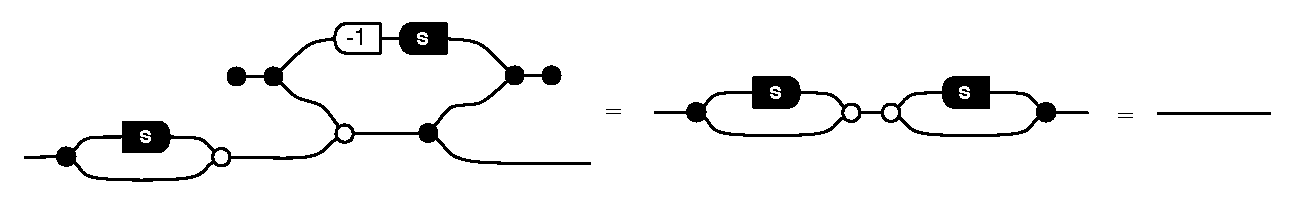
\includegraphics[height=1.2cm]{pics/exampleproof.pdf}$} 
\end{equation}

Note that~\eqref{eq:exampleproof} is \emph{not sound} for circuits
with our more liberal, operational semantics. Indeed, recall that when the
registers of~\eqref{eq:examplesfg} initially hold values $1$ and $2$, the input
$-1,1,-1,1,\dots$ results in the output $-2,2,-2,2,\dots$. This trajectory is
not permitted by a stateless wire, so $\ih_{k[s]}$ is not sound for reasoning
about LTI systems in general. The contribution of this paper is to provide sound
and complete theory to do just that.

In terms of the algebraic semantics, the difference from previous
work~\cite{BSZ1,BSZ3} is that where there streams were handled with Laurent
(formal power) series, here we use the aforementioned biinfinite streams.
Indeed, this is the very extension that allows us to discuss non-controllable
behaviours; in~\cite{BSZ1,BSZ3,Za,BE} all definable behaviours were
controllable. 

\paragraph{Structure of the paper.}
%We first review the prerequisite mathematical aspects. 
In \S\ref{sec.systems} we develop a categorical account of complete LTI discrete
dynamical systems. This serves as a denotational semantics for the graphical
language, introduced in \S\ref{sec.diagrams}, where we also derive the
equational characterisation. 
% This allows us to develop a signal flow calculus for
%these systems, and show that it is sound and complete.  
In we relate this to the operational semantics. We conclude  
in \S\ref{sec.control} with a structural account of controllability.


\section{Preliminaries}
We assume familiarity with basic concepts of linear algebra and category theory.

A \define{prop} is a strict symmetric monoidal category where the set of objects
is the natural numbers $\nn$, and monoidal product ($\oplus$) on objects is
addition. Homomorphism of props are identity-on-objects strict symmetric
monoidal functors.

A \define{symmetric monoidal theory} (SMT) is a presentation of a prop: a pair
$(\Sigma,E)$ where $\Sigma$ is a set of \define{generators} $\sigma\colon m\to
n$, where $m$ is the \define{arity} and $n$ the \define{coarity}. A
$\Sigma$-term is a obtained from $\Sigma$, identity $\idn\colon 1\to 1$ and
symmetry $\tw\colon 2\to 2$ by composition and monoidal product, according to
the grammar
\[
  \tm\ ::=\ \sigma\ |\ \idn\ |\ \tw\ |\ \tm\mathrel{;}\tm\ |\ \tm\oplus \tm 
\]
where $\mathrel{;}$ and $\oplus$ satisfy the standard typing discipline that
keeps track of the domains (arities) and codomains (coarities)
\[
\frac{\tm: m\to d \quad \tm': d\to n}
{\tm\mathrel{;}\tm': m\to n}
\quad
\frac{\tm: m\to n \quad \tm': m'\to n'}
{\tm\oplus \tm': m+m'\to n+n'}
\]
The second component $E$ of an SMT is a set of \define{equations}, where an
equation is a pair $(\tm,\mu)$ of $\Sigma$-terms with compatible types, i.e.
$\tm,\mu\colon m\to n$ for some $m,n\in\mathbb{N}$.

Given an SMT $(\Sigma,E)$, the prop $\mathbf{S}_{(\Sigma,E)}$ has as arrows the
$\Sigma$-terms quotiented by the smallest congruence that includes the laws of
symmetric monoidal categories and equations $E$. We sometimes abuse
notation by referring to $\mathbf{S}_{(\Sigma,E)}$ as an SMT. Given an arbitrary
prop $\mathbb{X}$, a \define{presentation} of $\mathbb{X}$ is an SMT
$(\Sigma,E)$ s.t.\ $\mathbb{X} \cong \mathbf{S}_{(\Sigma,E)}$.

String diagrams play an important role in our work. Given generators
$\Sigma$, we consider string diagrams to be arrows of
$\mathbf{S}_{(\Sigma,\varnothing)}$, that is, syntactic objects constructed by
composition from the generators, quotiented by the laws of symmetric monoidal
categories. For example, consider generators $2\to 1$ and $0\to 1$, which we
 draw below, with `dangling wires' accounting for 
arities and coarities:
\[
\addgen \quad \zerogen
\]
Armed with the graphical notation, we can present sets of equations as equations
between diagrams. For example, the SMT of commutative monoids consists of these
generators together with equations
\[
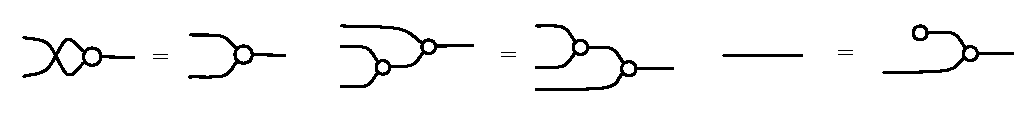
\includegraphics[height=.9cm]{pics/mon.pdf}
\]
that respectively are commutativity, associativity, and the unit law.

A \define{split mono} is a morphism $m\colon X\to Y$ such that there exists
$m'\colon Y\to X$ with $m'm=\idn_X$. 
For the remainder of the paper $\k$ is a field: for concreteness one may take
this to be the rationals $\mathbb{Q}$, the reals $\R$ or the booleans $\z_2$. 

\section{Linear time-invariant dynamical systems} \label{sec.systems}

This section focusses on the mathematical domains of interest for the remainder
of the paper. We rely on definitions of the \emph{behavioural approach} in
control, which is informed by compositional considerations~\cite{Wi}. The
concepts are standard in systems theory. Our categorical insights are, to the
best of our knowledge, original.

Following Willems~\cite{Wi3}, a \define{dynamical system} $(T, W,\bb)$ is: a
\define{time axis} $T$, a \define{signal space} $W$, and a \define{behaviour}
$\bb \subseteq W^T$. We refer to $w \in \bb$ as \define{trajectories}. 
%
In this paper we are interested in discrete trajectories that are
\define{biinfinite}: infinite in past and future.  Our time axis is thus the
integers $\z$. The signal space is $\k^d$, where $d$ is the number of
\define{terminals} of a system. These, in engineering terms, are the
interconnection variables that enable interaction with an environment.

The dynamical systems of concern to us are thus specified by some natural number
$d$ and a subset $\bb$ of $(\k^d)^\z$. The sets $(\k^d)^\z$ are $\k$-vector
spaces, with pointwise addition and scalar multiplication. We restrict attention
to \emph{linear} systems, meaning that $\bb$ is required to be a \emph{$\k$-linear subspace}---i.e.
closed under addition and multiplication by $\k$-scalars---of
$(\k^d)^\z$. 

We partition terminals into a \emph{domain} and \emph{codomain} of $m$ and $n$
terminals respectively, writing $\bb \subseteq (\k^m)^\z \oplus (\k^n)^\z \cong
(\k^d)^\z$.  This may seem artificial, in the sense that the assignment is
arbitrary.  In particular, it is crucial not to confuse the domains (codomains)
with inputs (outputs). In spite of the apparent contrivedness of choosing such a
partition, Willems and others have argued that it is vital for a sound theory of
system \emph{decomposition}; indeed, it enables the ``tearing'' of Willems'
tearing, zooming and linking~\cite{Wi}.
%. We
%use this structure to partition the system into a part we wish to connect to
%another system, and a part which we do not. It is an artifice in the sense that
%we may take any terminal in the domain and move it to the codomain, and vice
%versa. This ability is called compactness for a monoidal category.

Once the domains and codomains have been chosen, systems are linked by
connecting terminals. In models of physical systems this means variable coupling
or sharing~\cite{Wi}; in our discrete setting where behaviours are subsets of a
cartesian product---i.e.\ relations---it amounts to relational composition.
Since behaviours are both relations and linear subspaces, a central underlying
mathematical notion---as in previous work~\cite{BSZ1,BE}---is a linear relation. 
\begin{definition}
The monoidal category $\linrel_\k$ of $\k$-linear relations has $\k$-vector
spaces as objects, and as arrows from $V$ to $W$, linear subspaces of $V\oplus
W$, considered as $\k$-vector spaces.  Composition is relational: given $A\colon
U\to V$, $B\colon V\to W$, $A\mathrel{;}B\colon U\to W$ is the  relation
\[
  \left\{\,(u,w)\,\middle|\,\exists v\in V \textrm{ s.t. } \,(u,v)\in A \textrm{ and } (v,w)\in B\,\right\} 
\] 
that is easily checked to be a linear subspace. Finally, the monoidal product on both
objects and morphisms is direct sum.
\end{definition}


\smallskip
%The next restriction is the property of \define{time-invariance}. 
A behaviour is \define{time-invariant} when for every trajectory $w \in \bb$ and
any fixed $i\in\z$, the trajectory whose value at every time $t\in\z$ is
$w(t+i)$ is also in $\bb$.  
%
Time-invariance brings with it a connection with the algebra of polynomials.
Following the standard approach in control theory, going back to
Rosenbrock~\cite{Ro}, we work with polynomials over an indeterminate $s$ as well
as its formal inverse $s^{-1}$---i.e.\ the elements of the ring
$\pk$.\footnote{The introduction of the formal inverse $s^{-1}$ is a departure
from previous work~\cite{BSZ1,BSZ3} that dealt with Laurent streams (finite in
the past, infinite in the future), and algebraically with the field of
polynomial fractions. As we will see below, there is a natural action of $\pk$
on biinfinite streams, but it does not make sense, in general, to define the
action of a polynomial fraction on a biinfinite stream. }

The indeterminate $s$ acts on a given biinfinite stream $w \in \k^\z$ as a
one-step delay, and $s^{-1}$ as its inverse, a one step acceleration: 
\[ 
  (s\cdot w) (t) \Defeq w(t-1),\quad (s^{-1}\cdot w)(t) \Defeq w(t+1).
\]
We can extend this, in the obvious linear, pointwise manner, to an action of any
polynomial $p\in \pk$ on $w$.  Since $\k^\z$ is a $\k$-vector space, any such
$p$ defines a $\k$-linear map $\k^\z\to \k^\z$ ($w \mapsto p\cdot w$).

Given this, we can view $n\times m$ matrices over $\pk$ as $\k$-linear maps from
$(\k^m)^\z$ to $(\k^n)^\z$. This viewpoint can be explained succinctly as a functor from
the prop $\mat\pk$, defined below, to the category of $\k$-vector spaces and
linear transformations $\vect_\k$.

\begin{definition}
  The prop $\mat\pk$ has as arrows $m \to n$ the $n\times m$-matrices over
  $\pk$. Composition is matrix multiplication, and the monoidal product of $A$
  and $B$ is $\left[\begin{smallmatrix} A & 0 \\ 0 & B
  \end{smallmatrix}\right]$. The symmetries are permutation matrices.
\end{definition}

The functor of interest
\[
  \vectfun\maps \mat\pk \longrightarrow \vect_\k
\]
takes a natural number $n$ to $(\k^n)^\z$, and an $n\times m$ matrix to the
induced linear transformation $(\k^m)^\z \to (\k^n)^\z$. Note that $\vectfun$ is
faithful.

\smallskip
The final restriction on the set of behaviours is called \emph{completeness},
and is a touch more involved. For $t_0,t_1 \in \z$, $t_0 \le t_1$, write
$w|_{[t_0,t_1]}$ for the restriction of $w: \z \to \k^n$ to the set $[t_0,t_1] =
\{t_0, t_0+1, \dots, t_1\}$. Write  $\bb|_{[t_0,t_1]}$ for the set of the
restrictions of all trajectories $w \in \bb$ to $[t_0,t_1]$.  Then $\bb$ is
\define{complete} when $w|_{[t_0,t_1]} \in \bb|_{[t_0,t_1]}$ for all $t_0,t_1
\in \z$ implies $w \in \bb$. This topological condition is important as it
characterises the linear time-invariant behaviours that are kernels of the
action of $\mat\pk$; see Theorem \ref{thm.kernelreps}.

%We shall introduce one additional structure: a partition of the terminals of a
%dynamical system into two subsets, called a domain and a codomain. This will
%provide us with language to talk about interconnection of dynamical systems.
%We thus make the following definition.

\begin{definition}
  A \define{linear time-invariant (LTI) behaviour} comprises a domain
  $(\k^m)^\z$, a codomain $(\k^n)^\z$, and a subset $\bb \subseteq (\k^m)^\z
  \oplus (\k^n)^\z$ such that $(\z,\k^m \oplus \k^n,\bb)$ is a complete, linear,
  time-invariant dynamical system.
\end{definition}

The algebra of LTI behaviours is captured concisely as a prop.
\begin{proposition} \label{prop.ltidsiswelldefined}
  There exists a prop $\ltids$ 
  % objects the vector spaces of the form $(\k^n)^\z$ for $n \in \nn$, and 
  % morphisms $(\k^n)^\z \to (\k^m)^\z$ the LTIDS with domain
  with morphisms $m \to n$ the LTI behaviours with domain $(\k^m)^\z$ and
  codomain $(\k^n)^\z$. Composition is relational. The monoidal product is
  direct sum.
\end{proposition}

%\subsection{Kernel representations}


The proof of Proposition~\ref{prop.ltidsiswelldefined} relies on \emph{kernel
representations} of LTI  systems.  The following result lets us pass between
behaviours and polynomial matrix algebra.
%\[
%\mathfrak{B}:=\{w:\mathbb{Z} \rightarrow \k^q \mid \mbox{\rm s.t.~} R(\sigma,\sigma^{-1})w=0\}\; .
%\]
%and (for \emph{controllable} behaviors) the \emph{image representation}
%\begin{equation}\label{eq:im}
%w=M(\sigma,\sigma^{-1})\ell\; ,
%\end{equation}
%where $M\in\R^{q\times m}[s,s^{-1}]$, defining the behavior
%\[
%\mathfrak{B}:=\{w:\mathbb{Z} \rightarrow \R^q \mid  \mbox{\rm exists } \ell:\mathbb{Z}\rightarrow \R^m \mbox{\rm s.t. (\ref{eq:ker}) holds}\}\; ,
%\]}
%
%
\begin{theorem}[Willems {\cite[Th. 5]{Wi3}}] \label{thm.kernelreps}
  Let $\bb$ be a subset of $(\k^n)^\z$ for some $n \in \mathbb N$. Then $\bb$ is
  an LTI behaviour iff there exists $M \in
  \mat\pk$ such that $\bb = \mathrm{ker}(\vectfun M)$.
\end{theorem}

%Completeness is an important property. An example of a non-complete linear
%time-invariant subspace of $\k^\z$ is the set of all finitely supported
%functions $\z \to \k$.  This is not the kernel of the action of any matrix.

%\smallskip
The prop $\mat \pk$ is equivalent to the category $\fmod\pk$ of
finite-dimensional free $\pk$-modules. Since $\fmod R$ over a principal ideal
domain (PID) $R$ has finite colimits \cite{BSZ2}, and $\pk$ is a PID, $\mat \pk$
has finite colimits, and thus it has pushouts.

We can therefore define the prop $\cospan\mat\pk$ where arrows are (isomorphism
classes of) cospans of matrices: arrows $m \to n$ comprise a natural number
$d$ together with a $d\times m$ matrix $A$ and a $d\times n$ matrix $B$; we
write this $m\xrightarrow{A} d \xleftarrow{B}n$. Composition is given by
pushout, and isomorphic cospans are identified; for details see B\'enabou 
\cite{Be}.

%; see Appendix~\ref{app.cospans} for further details.

%Two cospans $m\xrightarrow{A} p
%\xleftarrow{B}n$, $m\xrightarrow{A'} q \xleftarrow{B'}n$ are equivalent when
%$p=g$ and there exists an invertible $p\times p$ matrix $U$ such that 
%\[
%\xymatrix@R=10pt{
%& p \ar[dd]^U \\
%m \ar[dr]_{A'} \ar[ur]^{A} & &  \ar[ul]_B n \ar[dl]^{B'} \\
%& p 
%}
%\]
%commutes: i.e. $A'=UA$ and $B'=UB$. 
%
%Composition in the category $\cospan\mat\pk$ is given by pushout of
%representatives of equivalence classes: if $m\xrightarrow{A} p
%\xleftarrow{B}n$ and $n\xrightarrow{C}q \xleftarrow{D}l$ are morphisms in
%$\cospan\mat\pk$, then  
We can then extend $\vectfun$ to the functor
\[
  \cospanfun \maps \cospan\mat\pk \longrightarrow \linrel_\k
\]
where on objects $\cospanfun(n)=\vectfun(n)=(\k^n)^\z$, and on arrows
%defined by mapping each cospan to a linear relation:
\[
  m\xrightarrow{A} d \xleftarrow{B}n
\]
maps to
\begin{equation}\label{eq.K}
  \big\{(\mathbf{x},\mathbf{y}) \,\big|\,
  (\vectfun A)\mathbf{x} = (\vectfun B)\mathbf{y}\big\} 
  \subseteq (\k^m)^\z \oplus (\k^n)^\z.
\end{equation}
It is straightforward to prove that this is well-defined.
%\begin{remark}\rm
%From a system theory point of view, the definition~\eqref{eq.K}, can be interpreted as associating with $R_1(\sigma,\sigma^{-1}), R_2(\sigma,\sigma^{-1})$, where 
%$R_i\in\R^{p\times n_i}[s,s^{-1}]$, the set of trajectories  
%\begin{multline}\label{eq:mycospan}
%\mathcal{Z}_{R_1,R_2}:= \\
%\{ w:\mathbb{Z}\rightarrow \k^{n_1+n_2} \mid 
%w=(w_1,w_2),\,
%R_1(\sigma,\sigma^{-1})w_1 = R_2(\sigma,\sigma^{-1})w_2 \}
%\end{multline}
%where $w=(w_1,w_2)$ is a terminal partition.
%\end{remark}
\begin{proposition}\label{prop.funct}
$\cospanfun$ is a functor.
\end{proposition}
\begin{proof}
Identities are clearly preserved; it suffices to show that composition is too.
Consider the diagram below, where the pushout is calculated in $\mat\pk$.
\[
\xymatrix{
  {}\ar[dr]_{A_1} & & \ar[dl]^{B_1}  
  \ar[dr]_{A_2} & & \ar[dl]^{B_2} {} 
 \\
& \ar[dr]_{C} & & \ar[dl]^{D}  \\
& & {\save*!<0cm,-.5cm>[dl]@^{|-}\restore}
}
\]
To show that $\cospanfun$ preserves composition we must verify that 
\begin{multline*}
\{(\mathbf{x},\mathbf{y})\,|\, \theta CA_1\mathbf{x} = \theta DB_2\mathbf{y}\}
= \\
\{(\mathbf{x},\mathbf{z})\,|\, \theta A_1\mathbf{x} = \theta B_1\mathbf{z}\} ; 
\{(\mathbf{z},\mathbf{y})\,|\, \theta A_2\mathbf{z} = \theta B_2\mathbf{y}\}.
\end{multline*}
The inclusion $\subseteq$ follows from properties of pushouts in $\mat\pk$ (see
\cite[Prop. 5.7]{BSZ2}).  To see $\supseteq$, we need to show that if there
exists $\mathbf{z}$ such that $\theta A_1\mathbf{x} = \theta B_1\mathbf{z}$ and
$\theta A_2\mathbf{z} = \theta B_2\mathbf{y}$, then $\theta CA_1\mathbf{x} =
\theta DB_2\mathbf{y}$.  But $\theta CA_1\mathbf{x}=\theta CB_1\mathbf{z}=\theta
DA_2\mathbf{z}=\theta DB_2\mathbf{y}$.
\end{proof}



%Paolo's original remark
%\begin{remark}\rm
%\textcolor{red}{The result of Prop. \ref{prop:Kfunct} can be interpreted from a system theory point of view as identifying with a terminal decomposition $w=(w_1,w_2)$ of the variables of a LTI behavior $\bb$ and associated kernel representation
%\begin{equation}\label{eq:ker}
%R_1(\sigma,\sigma^{-1})w_1=R_2(\sigma,\sigma^{-1})w_2\; ,
%\end{equation} 
%where $R_i\in\R^{p\times n_i}[s,s^{-1}]$, the set of trajectories 
%\begin{equation}\label{eq:mycospan}
%\mathcal{Z}_{R_1,R_2}:=\{z:\mathbb{Z}\rightarrow \R^p \mid \exists w_i:\mathbb{Z}\rightarrow \R^{n_i}\mbox{~s.t.~} z=R_i(\sigma,\sigma^{-1})w_i,~i=1,2\}\; .
%\end{equation}}
%\end{remark}

Rephrasing the definition of $\cospanfun$ on morphisms~\eqref{eq.K}, the
behaviour consists of those $(\mathbf{x},\mathbf{y})$ that satisfy
\[
  \vectfun\left[\begin{array}{cc} A & -B\end{array}\right]
  \left[\begin{array}{c}\mathbf{x}\\\mathbf{y}\end{array}\right] 
  = \mathbf{0},
\]
so one may say---ignoring for a moment the terminal domain/codomain assignment---that 
\[ 
  \cospanfun (\xrightarrow{A}\xleftarrow{B}) = \ker \vectfun\left[
  \begin{array}{cc} A & -B\end{array}\right].
\]

With this observation, as a consequence of Theorem~\ref{thm.kernelreps},
$\cospanfun$ has as its image (essentially) the prop $\ltids$. This proves
Proposition \ref{prop.ltidsiswelldefined}. We may thus consider $\cospanfun$ a
functor onto the codomain $\ltids$; denote this corestriction $\cospanfunrest$. We thus have a full functor:
\[
  \cospanfunrest \maps \cospan\mat\pk \longrightarrow \ltids.
\]

\begin{remark}\label{rmk:faithfulness}
It is important for the sequel to note that $\cospanfunrest$ is \emph{not} faithful.
For instance, $\cospanfunrest(1\xrightarrow{[1]}1\xleftarrow{[1]}1) =
\cospanfunrest(1\xrightarrow{ \left[\begin{smallmatrix} 1\\ 0\end{smallmatrix}\right]
}2 \xleftarrow{ \left[\begin{smallmatrix} 1\\ 0\end{smallmatrix}\right]} 1)$, yet
the cospans are not isomorphic. The task of the next section is to develop a
setting where these cospans are nonetheless \emph{equivalent}.
\end{remark}

\section{Presentation of $\ltids$} \label{sec.diagrams}
In this section we give a presentation of $\ltids$ as an SMT. This means 
that (\emph{i}) we obtain a syntax---conveniently expressed using string
diagrams---for specifying every LTI behaviour, and (\emph{ii}) a sound and
fully complete equational theory for reasoning about them.

\subsection{Syntax}
We start by describing the graphical syntax of dynamical systems, the arrows of
the category $\syntax = \mathbf{S}_{(\Sigma,\varnothing)}$, where $\Sigma$ is
the set of generators:
\begin{multline}\label{eq:generators}
\{
\addgen,
\zerogen,
\copygen,
\discardgen,
\delaygen, \\
\addopgen,
\zeroopgen,
\copyopgen,
\discardopgen,
\delayopgen
\} \\
\cup \{ \scalargen \mid a\in\k \,\} \cup \{ \scalaropgen \mid a\in\k \,\}
\end{multline}
For each generator, we give its \define{denotational semantics}, an LTI
behaviour, thereby defining a prop morphism $\llbracket - \rrbracket:
\syntax \to\ltids$.
\[
\addgen \!\!\mapsto \{\,( \left( 
  {\begin{smallmatrix}\tau \\ \upsilon\end{smallmatrix}} \right),\, \tau+\upsilon) \mid \tau,\upsilon \in \k^\z \,\}\maps 2\to 1
\]
\[
\quad
\zerogen \!\!\mapsto
\{\,((),0)\,\} \subseteq \k^\z\maps 0\to 1
\]
\[
\copygen \!\!\mapsto 
\{\, (\tau, \left( \begin{smallmatrix} \tau \\ \tau\end{smallmatrix} \right)) \mid \tau\in \k^\z \,\}\maps1\to 2
\]
\[
\quad
\discardgen \!\!\mapsto
\{\,(\tau,()) \mid \tau \in \k^\z\,\} \maps 1\to 0
\]
\[
\scalargen  \!\!\mapsto
\{\, (\tau, a\cdot\tau) \mid \tau\in\k^\z \, \} \maps 1 \to 1 \quad (a\in\k)
\]
\[
\ 
\delaygen \!\!\mapsto
\{\, (\tau, s\cdot\tau) \mid \tau\in\k^\z\,\} \maps 1 \to 1
\]

% In Fig.~\ref{fig:generators} we introduce half of the
%generators and their denotations.
%\begin{figure*}[ht]
%\[
%\addgen \!\!\mapsto \{\,( \left( 
%  {\begin{smallmatrix}\tau \\ \upsilon\end{smallmatrix}} \right),\, \tau+\upsilon) \mid \tau,\upsilon \in \k^\z \,\}\maps 2\to 1
%\]
%\[
%\quad
%\zerogen \!\!\mapsto
%\{\,((),0)\,\} \subseteq \k^\z\maps 0\to 1
%\]
%\[
%\copygen \!\!\mapsto 
%\{\, (\tau, \left( \begin{smallmatrix} \tau \\ \tau\end{smallmatrix} \right)) \mid \tau\in \k^\z \,\}\maps1\to 2
%\]
%\[
%\quad
%\discardgen \!\!\mapsto
%\{\,(\tau,()) \mid \tau \in \k^\z\,\} \maps 1\to 0
%\]
%\[
%\scalargen  \!\!\mapsto
%\{\, (\tau, a\cdot\tau) \mid \tau\in\k^\z \, \} \maps 1 \to 1 \quad (a\in\k)
%\]
%\[
%\ 
%\delaygen \!\!\mapsto
%\{\, (\tau, s\cdot\tau) \mid \tau\in\k^\z\,\} \maps 1 \to 1
%\]
%\caption{Generators and their denotations in $\ltids$. \label{fig:generators}}
%\end{figure*}
\noindent 
The denotations of the mirror image generators are the opposite relations.
Parenthetically, we note that a finite set of generators is possible
over a finite field, or the field $\mathbb{Q}$ of rationals, \emph{cf.}\
\S\ref{subsec:eqhopf}.

The following result guarantees that the syntax is fit for purpose: every
behaviour in $\ltids$ has a syntactic representation in $\syntax$.
\begin{proposition}\label{prop.syntaxfull}
  $\llbracket - \rrbracket: \syntax\to\ltids$ is full.
\end{proposition}
\begin{proof}
  The fact that $\llbracket - \rrbracket$ is a prop morphism is immediate since
  $\mathbb{S}$ is free on the SMT $(\Sigma,\varnothing)$ with no
  equations.  Fullness follows from the fact that $\llbracket - \rrbracket$
  factors as the composite of two full functors:
  \[
    \xymatrixrowsep{2pc}
    \xymatrix{
      \syntax \ar[d] \ar[dr]^{\llbracket-\rrbracket} \\
      \cospan\mat\pk \ar[r]_-{\cospanfunrest} & \ltids
    }
  \]
  The functor $\cospanfunrest$ is full by definition. The existence and fullness
  of the functor $\mathbb{S}\to\cospan\pk$ follows from \cite[Th. 3.41]{Za}. We
  give details in the next two subsections.
\end{proof}

Having defined the syntactic prop $\syntax$ to represent arrows in $\ltids$, our
task for this section is to identify an equational theory that
\emph{characterises} $\ltids$: i.e. one that is sound and fully complete. The
first step is to use the existence of $\cospanfun$: with the results
of~\cite{BSZ2,Za} we can obtain a presentation for $\cospan\mat\pk$. This is
explained in the next two subsections: in \S\ref{subsec:eqhopf} we present
$\mat\pk$ and in \S\ref{subsec:eqcospan}, the equations for cospans of matrices.

%%%%%%%%%%%%%%%%%%%%%%%%%%%%%%%%%%%%%%%%%%%%%%%%%%%%%%%%%%%

\subsection{Presentation of $\mat\pk$}\label{subsec:eqhopf}

%%%%%%%%%%%%%%%%%%%%%%%%%%%%%%%%%%%%%%%%%%%%%%%%%%%%%%%%%%%

To obtain a presentation of $\mat\pk$ as an SMT we only require 
some of the generators:
\begin{multline*}
\{
\addgen,
\zerogen,
\copygen,
\discardgen,
\delaygen,
\delayopgen\} \\
\cup \{ \scalargen \mid a\in\k \,\}
\end{multline*}
and the
% of
%Fig.\ref{fig:generators}, $\lower6pt\hbox{$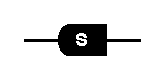
\includegraphics[height=0.6cm]{pics/delayop.pdf}$}$
%\[
%\{
%\lower8pt\hbox{$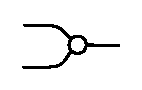
\includegraphics[height=0.7cm]{pics/add.pdf}$},
%\lower5pt\hbox{$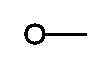
\includegraphics[height=0.5cm]{pics/zero.pdf}$},
%\lower8pt\hbox{$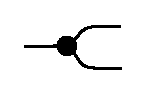
\includegraphics[height=0.7cm]{pics/copy.pdf}$},
%\lower5pt\hbox{$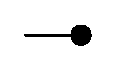
\includegraphics[height=0.5cm]{pics/discard.pdf}$},
%\lower6pt\hbox{$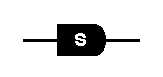
\includegraphics[height=0.6cm]{pics/delay.pdf}$},
%\lower6pt\hbox{$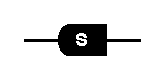
\includegraphics[height=0.6cm]{pics/delayop.pdf}$}
% \}
% \cup
% \{
% \lower6pt\hbox{$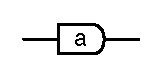
\includegraphics[height=0.6cm]{pics/scalar.pdf}$}
%\mid a \in \k\,
%\}
%\]
%and the 
following equations. %, see \cite{BSZ2,Za}. 
First, the white and the black structure forms a (bicommutative) bimonoid:
\[
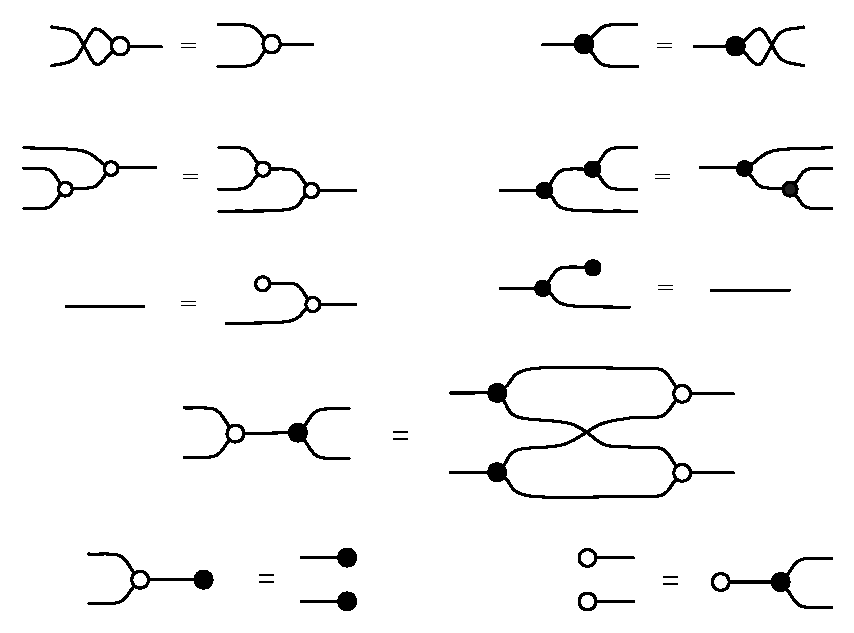
\includegraphics[width=.4\textwidth]{pics/bimonoid.pdf}
\]
Next, the formal indeterminate $s$ is compatible with the bimonoid structure
and has its mirror image as a formal inverse.
\[
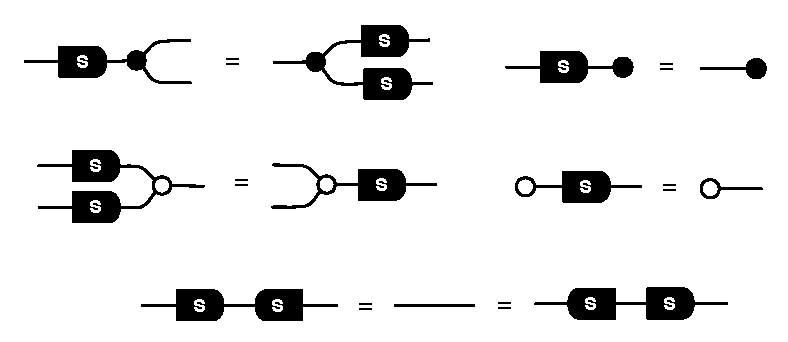
\includegraphics[height=3.1cm]{pics/s.pdf}
\]
Finally, we insist that the algebra of $\k$ be compatible with the bimonoid structure and commute with $s$.
%The equations below, in which $a,b\in\k$, are redundant if $\k=\mathbb{Q}$; instead,
%one needs an additional generator, the antipode, identified with the scalar
%$-1$. The details are not important; we merely mention that in other work we
%have used  
%\lower6pt\hbox{$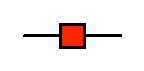
\includegraphics[height=0.6cm]{pics/antipode.pdf}$}
%to represent
%\lower6pt\hbox{$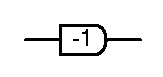
\includegraphics[height=0.6cm]{pics/minusone.pdf}$}, and that
%henceforward we adopt this convention.
\[
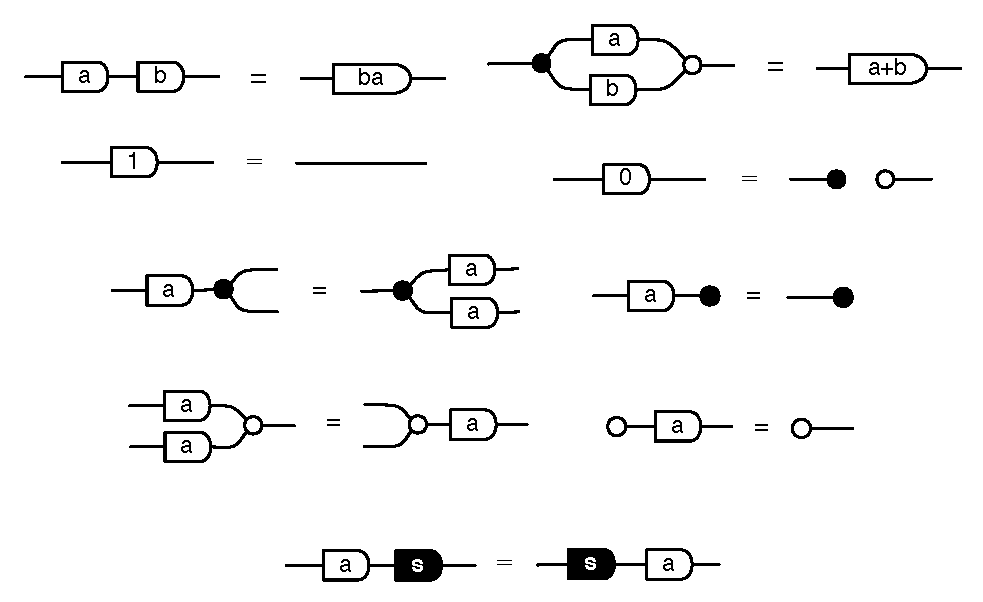
\includegraphics[height=5.3cm]{pics/scalars.pdf}
\]
The three sets of equations above form the theory of Hopf algebras. Write
$\ha_\pk$ for the prop induced by the SMT consisting of the equations
above. The following follows from~\cite[Prop.~3.9]{Za}.
\begin{proposition}
$\mat\pk\cong\ha_\pk$.
\end{proposition}

Arrows of $\mat\pk$ are matrices with polynomial entries, but it may not be
 obvious to the reader how polynomials arise with the string
diagrammatic syntax. We illustrate this below.

\begin{example}\label{rem:polys}
Any polynomial $p=\sum_{i=u}^v a_i s^i$, where $u\leq v\in\z$ and with
coefficients $a_i\in\k$, can be written graphically using the building blocks of
$\mathbb{HA}_\pk$. Rather than giving a tedious formal construction, we
illustrate this with an example for $\k=\R$. A term for $3s^{-3}-\pi
s^{-1}+s^{2}$ is:
\[
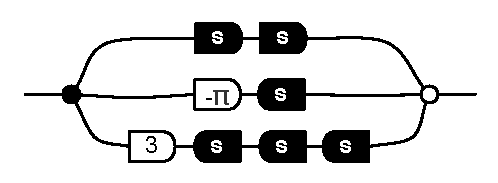
\includegraphics[height=1.7cm]{pics/polyex.pdf}
\]

As an arrow $1 \to 1$ in $\mat\pr$, the above term represents a $1\times
1$-matrix over $\pr$. To demonstrate how higher-dimensional matrices can be
written, we also give a term for the $2 \times 2$-matrix $\begin{bmatrix} 2 & 3s
  \\ s^{-1} & s+1 \end{bmatrix}$:
\[
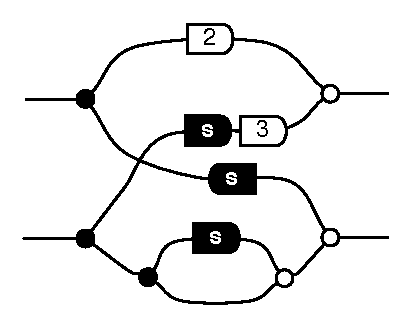
\includegraphics[height=3cm]{pics/exmatrix.pdf}
\]
The above examples are intended to be suggestive of a normal form for terms in
$\ha_\pk$; for further details see \cite{Za}.
\end{example}

%%%%%%%%%%%%%%%%%%%%%%%%%%%%%%%%%%%%%%%%%%%%%%%%%%%%%%%%%%%%%%%%%%%%

\subsection{Presentation of $\cospan\mat\pk$\label{subsec:eqcospan}}

%%%%%%%%%%%%%%%%%%%%%%%%%%%%%%%%%%%%%%%%%%%%%%%%%%%%%%%%%%%%%%%%%%%%

To obtain the equational theory of $\cospan\mat \pk$ we need the full set of
generators~\eqref{eq:generators},
%\begin{gather*}
%\{
%\lower8pt\hbox{$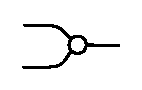
\includegraphics[height=0.7cm]{pics/add.pdf}$},
%\lower5pt\hbox{$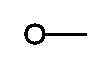
\includegraphics[height=0.5cm]{pics/zero.pdf}$},
%\lower8pt\hbox{$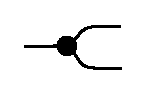
\includegraphics[height=0.7cm]{pics/copy.pdf}$},
%\lower5pt\hbox{$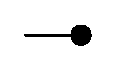
\includegraphics[height=0.5cm]{pics/discard.pdf}$}
% \}
% \cup
% \{
% \lower6pt\hbox{$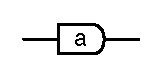
\includegraphics[height=0.6cm]{pics/scalar.pdf}$}
%\mid a \in \k\,
%\} \;\cup \\
%\{
%\lower8pt\hbox{$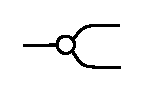
\includegraphics[height=0.7cm]{pics/addop.pdf}$},
%\lower5pt\hbox{$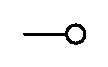
\includegraphics[height=0.5cm]{pics/zeroop.pdf}$},
%\lower8pt\hbox{$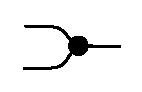
\includegraphics[height=0.7cm]{pics/copyop.pdf}$},
%\lower5pt\hbox{$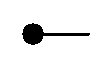
\includegraphics[height=0.5cm]{pics/discardop.pdf}$}
% \}
% \cup
% \{
% \lower6pt\hbox{$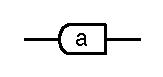
\includegraphics[height=0.6cm]{pics/scalarop.pdf}$}
%\mid a \in \k\,
%\}  \;\cup \\
%\{
%\lower6pt\hbox{$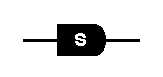
\includegraphics[height=0.6cm]{pics/delay.pdf}$},
%\lower6pt\hbox{$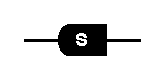
\includegraphics[height=0.6cm]{pics/delayop.pdf}$}
%\}
%\end{gather*}
along with the equations of $\ha_\pk$, their mirror images, and the
following
\[
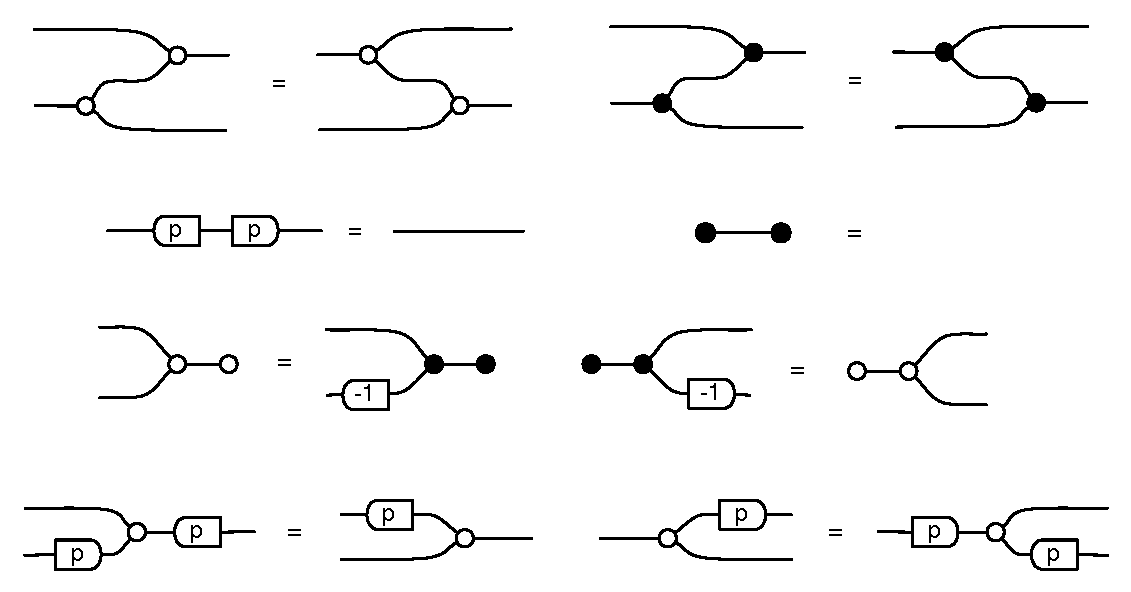
\includegraphics[height=4cm]{pics/cospan.pdf}
\]
where $p$ ranges over the nonzero elements of $\pk$ (see
Example~\ref{rem:polys}). Note that in the second equation on the right-hand
side, we use the so-called `empty diagram', or blank space, to represent the
identity map on the monoidal unit, 0. 

The equations of $\ha_\pk$ ensure the generators of $\ha_\pk$ behave as
morphisms in $\mat\pk$, while their mirror images ensure the remaining
generators behave as morphisms in the opposite category $\mat\pk^{\mathrm{op}}$.
The additional equations above govern the interaction between these two sets of
generators, axiomatising pushouts in $\mat\pk$.
%
Let $\ihcsp$ denote the resulting SMT.
The procedure for obtaining the equations from a distributive law of props 
is explained in~\cite[\S{3.3}]{Za}.
\begin{proposition}[Zanasi~{\cite[Th.~3.41]{Za}}]\label{prop:cospanpresentation}
\[\cospan \mat\pk \cong \ihcsp.\]
\end{proposition}

Using Prop.~\ref{prop:cospanpresentation} and the existence of $\cospanfunrest$,
%\[
%  \cospanfun \maps \cospan\mat\pk \longrightarrow \ltids
%\]
the equational theory of $\ihcsp$ is a sound proof system for reasoning about
$\ltids$. Due to the fact that $\cospanfunrest$ is not faithful (see
Remark~\ref{rmk:faithfulness}), however, the system is not complete. Achieving
completeness is our task for the remainder of this section.

%%%%%%%%%%%%%%%%%%%%%%%%%%%%%%%%%%%%%%%%%%%%%%%%%%%%%%%%%

\subsection{Corelations}

%%%%%%%%%%%%%%%%%%%%%%%%%%%%%%%%%%%%%%%%%%%%%%%%%%%%%%%%%

%We have already discussed the fact that $\mat\pk$ has finite colimits. 
%Moreover,

In the category of sets, relations can be identified with jointly-monic spans of
functions; that is, those spans $X\xleftarrow{p}R\xrightarrow{q}Y$ where the
induced map $R\xrightarrow{\langle p,q\rangle}X\times Y$ is injective.
Corelations are a dual concept: we consider cospans
$X\xrightarrow{i}S\xleftarrow{j}Y$ where the induced map
$X+Y\xrightarrow{[i,j]}S$ is surjective. To make sense of this more generally,
one needs a category with a factorisation system. 
%(See Appendix~\ref{app.factorisation} for a definition.)  
In this subsection we
identify a factorisation system in $\mat\pk$, and show that the induced prop
$\corel\mat\pk$ of corelations is isomorphic to $\ltids$.  We then give a
presentation of $\corel\mat\pk$ and arrive at a sound and fully complete
equational theory for $\ltids$.

%Every morphism in $\mat\pk$ admits a factorisation into an epi followed
%by a split mono. 
%%In this section we show that this factorisation occurs in a functorial way. 
%This will allow us to define a PROP of \emph{corelations}
%$\corel \mat \pk$.

\begin{proposition}\label{prop.matfactorisation}
  Every morphism $R \in \mat\pk$ can be factored as $R = BA$, where $A$ is an
  epi and $B$ is a split mono.
\end{proposition}
\begin{proof}
%We use the Smith normal form~\cite[Section~6.3]{Ka}. 
%
Given any matrix $R$, the Smith normal form~\cite[Section~6.3]{Ka}  gives
  us  $R = VDU$, where $U$ and $V$ are invertible, and $D$
  is diagonal. In graphical notation we can write it thus:
  \[
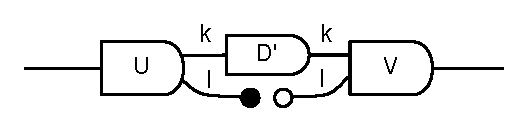
\includegraphics[height=1.1cm]{pics/smith1.pdf}
  \]
  This implies we may write it as $R = U';D';V'$, where $U'$ is a split
  epimorphism, $D'$ diagonal of full rank, and $V'$ a split monomorphism.
  Explicitly, the construction is given by
  \[
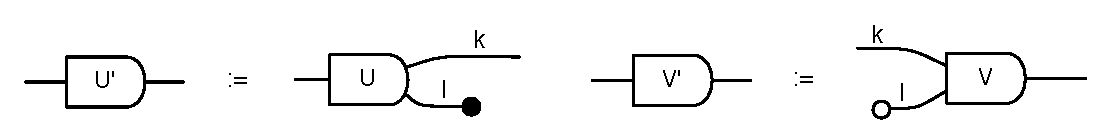
\includegraphics[height=1cm]{pics/uv.pdf}
  \]
  Recall that $\pk$ is a PID, so the full rank diagonal matrix $D'$ is epi. It
  can be checked that $R = V'(D'U')$ is an epi-split mono factorisation. 
%In Appendix~\ref{app.prop.matfactorisation}.
\end{proof}
A more careful examination of Proposition~\ref{prop.matfactorisation} yields:

\begin{corollary} \label{cor.episplitmono}
  Let $\mathcal E$ be the subcategory of epis and
  $\mathcal M$ the subcategory of split monos. The pair $(\mathcal
  E,\mathcal M)$ is a factorisation system on $\mat\pk$, with $\mathcal M$
  stable under pushout.
\end{corollary}
%\begin{proof}
%In Appendix~\ref{app.cor.episplitmono}. See Appendix~\ref{app.factorisation} for background.
%\end{proof}

%The remainder of this section is devoted to proving this proposition. To begin,
%note that both these subcategories contain all isomorphisms of $\mat\pk$. Next,
%observe that every matrix can indeed be factored as required.

%It remains to prove property (iii): functoriality. We derive this from the
%functoriality of a factorisation system on $\vect$. For this, we need the
%following fundamental result. 

%\begin{proposition}[Willems {\cite[p.565]{Wi3}}] \label{prop.magic}
%  Let $M,N$ be matrices in $\mat\pk$. Then $\ker \vectfun M \subseteq \ker \vectfun N$ if and
%  only if there exists a matrix $X$ such that $M;X = N$.
%\end{proposition}

%We also use the following straightforward observation.
%\begin{lemma}[Willems {\cite[p.576]{Wi3}}] \label{lem.surjective}
%  Let $p \in \pk$. Then the linear map $\vectfun(p): \k^\z \to \k^\z$ is an
%  epimorphism.
%\end{lemma}

%\begin{proof}[Proposition \ref{prop.fact}]
%  Let $R \in \mat\pk$ factor as $R= (U';D');V'$ as above. Note that as $U'$ and
%  $V'$ are split epi and split mono respectively, $\vectfun U'$ and $\vectfun V'$ are
%  too, and hence a fortiori epi and mono respectively.  Moreover, $\vectfun D'$ is
%  epi as it acts streamwise on $(k^n)^\z$, and by Lemma \ref{lem.surjective} the
%  action on each stream is a surjective linear map. Thus $\vectfun R = \vectfun
%  (U';D');\vectfun V'$ is an epi-mono factorisation of $\vectfun R$ in Vect. 
%
%  Now $\vect$ is an abelian category, and so has an epi-mono factorisation
%  system \cite{ML}. We will use Proposition \ref{prop.magic} to show the
%  functoriality of the epi-mono factorisation system in $\vect$ implies the
%  functoriality of the epi-splitmono system in $\mat\pk$. To that end, suppose we
%  have matrices $R$, $R'$, $A$, $B$ such that $R;B = A;R'$ and such that we have
%  epi-splitmono factorisations $R = E;M$ and $R' = E';M'$. Then $\vectfun R = \vectfun
 % E;\vectfun M$, $\vectfun R' = \vectfun E';\vectfun M'$ are epi-mono factorisations in
 % $\vect$, so there exists a unique linear map $\xi$ such that
 % \begin{equation} \label{eq.funvect}
 %   \begin{aligned}
 %     \xymatrixcolsep{3pc}
 %     \xymatrixrowsep{3pc}
 %     \xymatrix{
%	\ar[r]^{\vectfun E} \ar[d]_{\vectfun A} & \ar[r]^{\vectfun M}
%	\ar@{.>}[d]^{\exists! \xi} &  \ar[d]^{\vectfun B} \\
%	\ar[r]_{\vectfun E'}& \ar[r]_{\vectfun M'} & 
%      }
%    \end{aligned}
%  \end{equation}
%  commutes. This implies $\ker \vectfun E$ is contained in $\ker \vectfun A; \vectfun
%  E'$, so Proposition \ref{prop.magic} implies we have a matrix $X$ such that $E;X
%  = A;E'$. As $E;M;B = R;B = A;R'= A;E';M'$, this further implies that $E;M;B =
%  E;X;M'$, and as $E$ is epi this gives $M;B = X;M'$. Thus $X$ makes the
%  functoriality diagram commute.
%
%  Since $\xi$ is the unique such map that makes (\ref{eq.funvect}) commute, we
%  then have $\theta X = \xi$. By the faithfulness of $\theta$, $X$ is then unique.
%  This proves functoriality.
%\end{proof}

Given finite colimits and an $(\mathcal E,\mathcal M)$-factorisation system with
$\mathcal M$ stable under pushouts, we may define a category of corelations. The
morphisms are isomorphism classes of cospans $X \xrightarrow{i} S \xleftarrow{j}
Y$ where the copairing $[i,j]\maps X+Y \to S$ is in $\mathcal E$.  Composition
is given by pushout, as in the category of cospans, followed by factorising the
copairing of the resulting cospan. This is a dualisation of the well-known
construction of relations from spans~\cite{JW}; further details can be found
in~\cite{Fo}.


\begin{definition}
  The prop $\corel \mat \pk$ has as morphisms equivalence classes of
  jointly-epic cospans in $\mat\pk$.  
  %Composition is given by the jointly-epic part of the pushout.
\end{definition}

We have a full morphism
\[
  F\maps \cospan \mat \pk \longrightarrow \corel \mat \pk
\]
mapping a cospan to its jointly-epic counterpart given by the
 factorisation system. %We will show that 
Then $\cospanfunrest$
factors through $F$ as follows:
\[
  \xymatrixrowsep{2pc}
  \xymatrix{
    \cospan\mat\pk \ar[d]_F \ar[dr]^{\cospanfunrest} \\
    \corel\mat\pk \ar[r]_-{\Phi} & \ltids
  }
\]
The morphism $\Phi$ along the base of this triangle is an isomorphism of props, 
and this is our main technical result, Theorem~\ref{thm.main}. The proof relies
on the following beautiful result of systems theory.

\begin{proposition}[Willems {\cite[p.565]{Wi3}}] \label{prop.magic}
  Let $M,N$ be matrices over $\pk$. Then $\ker \vectfun M \subseteq \ker \vectfun N$ iff $\exists$ a matrix $X$ s.t.\ $XM = N$.
\end{proposition}

Further details and a brief history of the above proposition can be found in
Schumacher \cite[pp.7--9]{Sc}. 

\begin{theorem}\label{thm.main}
  There is an isomorphism of props 
  \[
    \Phi\maps \corel\mat\pk \longrightarrow \ltids
  \]
  taking a corelation $\xrightarrow{A}\xleftarrow{B}$ 
  to $\cospanfunrest(\xrightarrow{A}\xleftarrow{B}) = {\ker\theta [A \ -B]}$.
  %mapping each natural number $n$ to the space $(\k^n)^\z$ and each corelation
  %\[
  %  n \stackrel{f}\longrightarrow a \stackrel{g}\longleftarrow m
  %\]
  %to the difference kernel $\ker\vectfun (f\ -g)$.
\end{theorem}
\begin{proof}
  For functoriality, start from $\vectfun\maps\mat\pk \to
  \vect_\k$. Now (i) $\vect_k$ has an epi-mono factorisation system, (ii)
  $\vectfun$ maps epis to epis and (iii) split monos to monos, so $\vectfun$
  preserves factorisations. Since it is a corollary of Prop. \ref{prop.funct}
  that $\theta$ preserves colimits, it follows that $\vectfun$ extends to
   $\Psi\maps\corel\mat\pk \to \corel\vect_\k$. But $\corel\vect_\k$ is
  isomorphic to $\linrel_\k$ (see %Appendix \ref{app.corellinrel} and~
  \cite{Fo}).
  By Theorem \ref{thm.kernelreps}, the image of $\Psi$ is $\ltids$, and taking
  the corestriction to gives us precisely $\Phi$, which is therefore a full
  morphism of props.

  As corelations $n \to m$ are in one-to-one correspondence with epis out of
  $n+m$, to prove faithfulness it suffices to prove that if two epis $R$ and $S$
  with the same domain have the same kernel, then there exists an invertible
  matrix $U$ such that $UR =S$. This is immediate from
  Proposition~\ref{prop.magic}: if $\ker R= \ker S$, then we can find $U, V$
  such that $UR = S$ and $VS = R$. Since $R$ is an epimorphism, and since $VUR =
  VS = R$, we have that $VU=1$ and similarly $UV =1$. This proves that any two
  corelations with the same image are isomorphic, and so $\Phi$ is full and
  faithful.  
\end{proof}

%%%%%%%%%%%%%%%%%%%%%%%%%%%%%%%%%%%%%%%%%%%%

\subsection{Presentation of $\corel\mat\pk$}

%%%%%%%%%%%%%%%%%%%%%%%%%%%%%%%%%%%%%%%%%%%%

Thanks to Theorem~\ref{thm.main}, the task of obtaining a presentation of $\ltids$
is that of obtaining one for $\corel\mat\pk$. 
%One way to do this is to focus on the full morphism $F$ from cospans to corelations.
%\[
%  \cospan \mat \pk \longrightarrow \corel \mat \pk.
%\]
%
To do this, we start with the presentation
$\mathbb{IH}^{\textsf{Csp}}$ for $\cospan\mat\pk$ of \S\ref{subsec:eqcospan}; the task of
this section is to identify the additional equations that equate
exactly those cospans that map via $F$ to the same corelation.
%; i.e. those cospans $c,c'$ for which $Fc=Fc'$.  

%As such, our task 
%now is to understand the conditions under which two cospans have the same 
%jointly-epic parts.

In fact, only one new equation is required, the ``white bone law'':
\begin{equation}\label{eq.whitebone}
  \lower8pt\hbox{$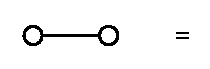
\includegraphics[height=.7cm]{pics/wbone.pdf}$}\qquad\qquad
\end{equation}
where we have carefully drawn the empty diagram to the right of the equality symbol.
Expressed in terms of cospans, \eqref{eq.whitebone} asserts that  
$0\rightarrow 1\leftarrow 0$ and $0\rightarrow 0\leftarrow 0$ are identified:
indeed, the two clearly yield the same corelation. The intuition here is that
cospans $X \xrightarrow{i} S \xleftarrow{j} Y$ map to the same corelation if their
respective copairings $[i,j]\maps X+Y \to S$ have the same jointly-epic parts.
More colloquially, this allows us to `discard' any part of the cospan that is
not connected to the terminals. This is precisely what \eqref{eq.whitebone}
represents. Further details on this viewpoint can be found in \cite{CF}. 
%

Let $\mathbb{IH}^{\mathsf{Cor}}$ be the SMT obtained
from the equations of $\mathbb{IH}^{\mathsf{Csp}}$ together with equation~\eqref{eq.whitebone}.
\begin{theorem}
$\corel \mat \pk \cong \mathbb{IH}^{\mathsf{Cor}}$.
\end{theorem}
\begin{proof}
Since equation~\eqref{eq.whitebone} holds in $\corel\mat\pk$, we have
a full morphism $\ihcor \to \corel\mat\pk$; it remains
to show that it is faithful. It clearly suffices to show that in the equational
theory $\ihcor$ one can prove that every cospan is equal
to its corelation. Suppose then that $m \xrightarrow{A} k \xleftarrow{B} n$ is a cospan
and $m \xrightarrow{A'} k' \xleftarrow{B'} n$ its corelation. Then, by definition, 
there exists a split mono $M\maps k'\to k$ such that $MA'=A$ and $MB'=B$. Moreover, by the construction
of the epi-split mono factorisation in $\mat\pk$, $M$ is of the form $\lower10pt\hbox{$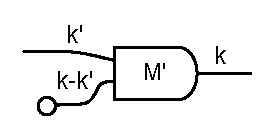
\includegraphics[height=1cm]{pics/m.pdf}$}$ where $M'\maps k\to k$ is invertible. We can now give the derivation
in $\mathbb{IH}^{\mathsf{Cor}}$:
\begin{align*}
\lower7pt\hbox{$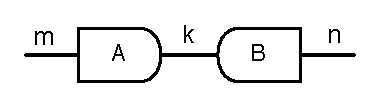
\includegraphics[height=.7cm]{pics/cospan1.pdf}$} \quad
&\stackrel{\ihcsp}{=} \quad
\lower10pt\hbox{$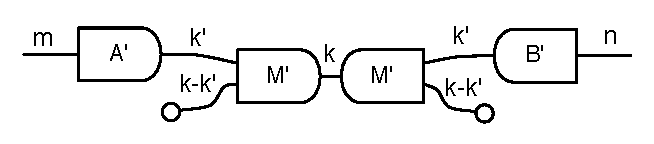
\includegraphics[height=1cm]{pics/cospan2.pdf}$} \\
\quad &\stackrel{\ihcsp}{=} \qquad 
\lower8pt\hbox{$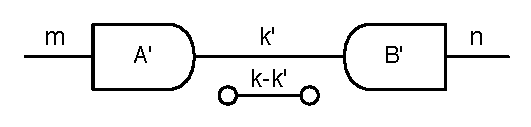
\includegraphics[height=.8cm]{pics/cospan3.pdf}$} \\
&\stackrel{\eqref{eq.whitebone}}{=} \qquad\qquad
\lower7pt\hbox{$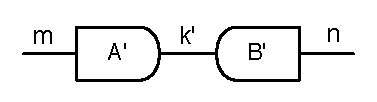
\includegraphics[height=.7cm]{pics/cospan4.pdf}$}
\end{align*}
\end{proof}


%The new construction rule we have for axioms is that we may replace split-monic
%matrices followed by a cozero with just a cozero. Split monic matrices are just
%the tensor of identity and zero matrices followed by an invertible matrix. The
%rules to see that an invertible matrix followed by a cozero is equal to a cozero
%already exist. So the only additional rule is that a zero followed by a cozero
%is a $0 \to 0$ cozero: ie. nothing. This is the bone law.
%\[
%  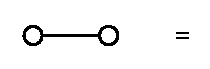
\includegraphics[height=.7cm]{pics/wbone.pdf}
%\]
%For the reader's convenience, we collect all the equations in Appendix~\ref{app.equations}%
%
%Thus a cospan may be reduced to its jointly-epic part by repeated application of
%the usual laws and the white bone law.  Moreover, two cospans then have the same
%jointly-epic part if and only if the are the same up to such applications.

We therefore have a sound and fully complete equational theory for LTI systems,
and also a normal form for each LTI system: every such system can be written, in
an essentially unique way, as a jointly-epic cospan of terms in $\ha_\pk$ in
normal form.

\begin{remark} \label{rmk.omittedaxs}
 $\ihcor$ %(summarised in Appendix~\ref{app.equations}) 
 can also be described as having the equations of $\ih_\pk$~\cite{BSZ2,Za}, but
\emph{without} $\!\!\lower4pt\hbox{$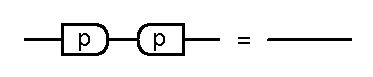
\includegraphics[height=.5cm]{pics/badequation.pdf}$}$,
and related $\!\lower7pt\hbox{$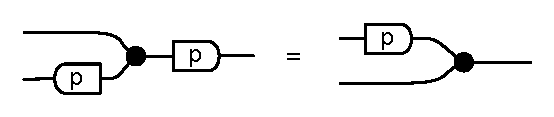
\includegraphics[height=.8cm]{pics/badequation2.pdf}$}$
and $\!\lower7pt\hbox{$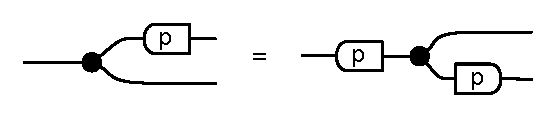
\includegraphics[height=.8cm]{pics/badequation3.pdf}$}$.
Our results generalise; given any PID $R$ we have (informally speaking):
\begin{align*}
  \ihcor_R &= \ih_R -
  \left\{
    \begin{array}{c}
      \lower6pt\hbox{$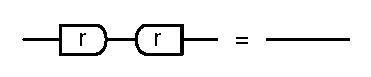
\includegraphics[height=.6cm]{pics/badequationgen.pdf}$}, \\
      \lower7pt\hbox{$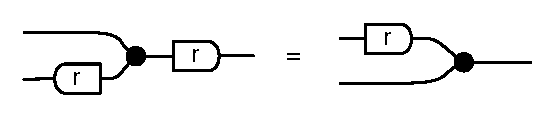
\includegraphics[height=.7cm]{pics/badequation2gen.pdf}$},\\
      \lower7pt\hbox{$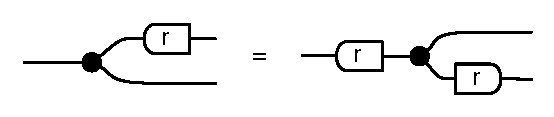
\includegraphics[height=.7cm]{pics/badequation3gen.pdf}$}
    \end{array}
    \middle|\,r\neq 0\in R\,
  \right\} \\
  &\cong \corel \mat R
\end{align*}
and, because of the transpose duality of matrices:
\begin{align*}
  \ih^{\mathsf{Rel}}_R &= \ih_R - 
  \left\{
    \begin{array}{c} 
      \lower6pt\hbox{$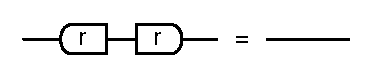
\includegraphics[height=.6cm]{pics/goodequationgen.pdf}$},\\
      \lower7pt\hbox{$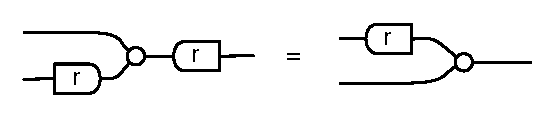
\includegraphics[height=.7cm]{pics/goodequation2gen.pdf}$}, \\
      \lower7pt\hbox{$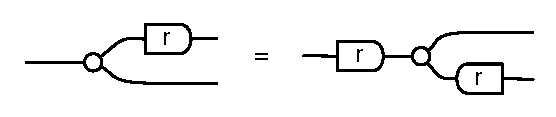
\includegraphics[height=.7cm]{pics/goodequation3gen.pdf}$}
    \end{array}
    \middle|\,r\neq 0\in R\,
  \right\}\\
  &\cong \mathsf{Rel} \mat R.
\end{align*}
\end{remark}

\begin{remark}\label{rmk:splus1}
The omitted equations each associate a cospan
with a span that, in terms of behaviour, has the effect of passing to a 
sub-behaviour\footnote{In fact the `largest controllable sub-behaviour' of the system. We explore 
controllability in Section \ref{sec.control}.}.
Often this is a strict sub-behaviour, hence the failure of soundness of $\ih$ identified in the introduction. 

For example, consider the system $\mathcal B$ represented by the cospan
\[
\lower6pt\hbox{$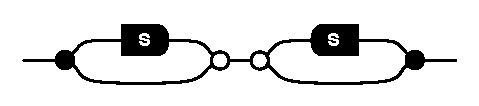
\includegraphics[height=.8cm]{pics/splus1.pdf}$}
\]
We met this system in the introduction; indeed the following
derivation can be performed in $\ihcor$:
\[
\includegraphics[height=1.3cm]{pics/firstequality.pdf}
\]
 The trajectories are $w= (w_1, w_2) \in \k^\z \oplus \k^\z$ where
$(s+1)\cdot w_1= (s+1)\cdot w_2$; that is, they satisfy the difference equation
\[ 
w_1(t-1)+w_1(t)-w_2(t-1)-w_2(t)=0.  
\]
As we saw in the introduction, however, an equation of $\ih_{\k[s]}$ omitted from
$\ihcor_{\k[s,s^{-1}]}$ equates this to the identity system $\id$, with the
identity behaviour those sequences of the form $w = (w_1,w_1) \in \k^\z \oplus
\k^\z$.  The identity behaviour is strictly smaller than $\mathcal B$; e.g., $\mathcal B$ contains $(w_1,w_2)$ with $w_1(t) = (-1)^t$
and $w_2(t) =0$.
\end{remark}

The similarity between our equational presentations of $\ihcor_{\k[s,s^{-1}]}$ and that of
 $\ih_{\k[s]}$  given in~\cite{BSZ1,BSZ3} is remarkable,
considering the differences between the intended semantics of signal flow graphs
that string diagrams in those theories represent, as well as the underlying mathematics
of streams, which for us are elements of the $\k$ vector space $\k^{\mathbb{Z}}$ and
in~\cite{BSZ1,BSZ3} are Laurent series. We contend that this is evidence of the \emph{robustness}
of the algebraic approach: the equational account of how various components of signal
flow graphs interact is, in a sense, a higher-level specification than the technical details of the underlying
mathematical formalisations.

\section{Controllability} \label{sec.control}

Suppose we are given a current and a target trajectory for a system. Is it
always possible, in finite time, to steer the system onto the target trajectory? If so, the 
 system is deemed controllable, and the problem of controllability of systems is at
the core of control theory. The following definition is due to
Willems~\cite{Wi2}.

\begin{definition}\label{def:contr}
A system $(T,W,\bb)$ (or simply the behaviour $\bb$) is \define{controllable} if
for all $w,w' \in \bb$ and all times $t_0\in\mathbb{Z}$, there exists $w'' \in
\bb$ and $t_0^\prime\in\mathbb{Z}$ such that $t_0'>t_0$ and $w''$ obeys
\[
  w''(t) = 
  \begin{cases} 
    w(t) & t \le t_0 \\
    w'(t-t_0') & t \ge t_0'.
  \end{cases}
\]
\end{definition}
%$\bb$ is controllable if given the past of some trajectory and the future of
%another, there exists a trajectory in the behaviour that transitions, in finite
%time, from the chosen past to the chosen future. 

As mentioned previously, a novel feature of our graphical calculus is
that it allows us to consider non-controllable behaviours.

\begin{example} \label{ex.noncontrol}
Consider the system in the introduction, further elaborated in Remark~\ref{rmk:splus1}.
%represented by the signal flow
%graph~\eqref{eq:examplesfg}. The equation 
%\[
%\includegraphics[height=1.3cm]{pics/firstequality.pdf}
%\]
%follows from the equations of $\ltids$, and so as an $\ltids$ system
%\eqref{eq:examplesfg} is the system represented by the corelation
%%\[
%$1 \xrightarrow{[s+1]} 1 \xleftarrow{[s+1]} 1.$
%%\]
%
%As discussed in Remark \ref{rmk.omittedaxs}, 
As noted previously,
the trajectories of this system are
precisely those sequences $w= (w_1, w_2) \in \k^\z \oplus \k^\z$ that satisfy
the difference equation
\[
  w_1(t-1)+w_1(t)-w_2(t-1)-w_2(t)=0.
\]
To see that the system is non-controllable, note that
\[
  w_1(t-1)-w_2(t-1) = -(w_1(t)-w_2(t)),
\]
so $(w_1-w_2)(t) = (-1)^tc_w$ for some $c_w \in \k$. This $c_w$ is a time-invariant
property of any trajectory. Thus if $w$ and $w'$ are trajectories such that $c_w \ne
c_{w'}$, then it is not possible to transition from the past of $w$ to the
future of $w'$ along some trajectory in $\mathcal B$. 

Explicitly, taking $w(t) = ((-1)^t,0)$ and $w'(t) = ((-1)^t2,0)$ suffices to
show $\mathcal B$ is not controllable.
\end{example}

\subsection{A categorical characterisation}
We now show that controllable systems are precisely those representable as
\emph{spans} of matrices. This novel characterisation leads to new ways of
reasoning about controllability of composite systems. 

Among the various equivalent conditions for controllability, the existence of
\emph{image representations} is most useful for our purposes.
\begin{proposition}[Willems {\cite[p.86]{Wi}}] \label{thm.imagereps}
  An LTI behaviour $\bb$ is controllable iff $\exists\; M \in \mat\pk$ such that $\bb = \im \theta M$.
\end{proposition}

Restated in our language, Prop. \ref{thm.imagereps} states that controllable
systems are precisely those representable as \emph{spans} of matrices. 

\begin{theorem} \label{cor.spanreps}
  Let $m \xrightarrow{A} d \xleftarrow{B} n$ be a corelation in $\corel\mat\pk$. Then
  $\Phi(\xrightarrow{A}\xleftarrow{B})$ is controllable iff $\exists$ $R: e \to m$, $S: e\to n$ s.t.
  \[
    m \xleftarrow{R} e \xrightarrow{S} n = m \xrightarrow{A} d \xleftarrow{B} n
  \]
  as morphisms in $\corel\mat\pk$. 
\end{theorem}
\begin{proof}
  To begin, note that the behaviour of a span is its joint image. That is,
  $\Phi(\xleftarrow{R}\xrightarrow{S})$ is the composite of linear
  relations $\ker\vectfun[\mathrm{id}_m \; -R]$ and $\ker\vectfun[S\;
  -\mathrm{id}_n]$, which comprises all $(\mathbf{x},\mathbf{y}) \in (\k^m)^\z
  \oplus (\k^n)^\z$ s.t.\ $\exists$ $\mathbf{z} \in (\k^e)^\z$ with
  $\mathbf{x} = \vectfun R \mathbf{z}$ and $\mathbf{y} = \vectfun S
  \mathbf{z}$. Thus
  \[
    \Phi(\xleftarrow{R}\xrightarrow{S}) = \im \vectfun \left[
    \begin{matrix} R \\ S \end{matrix} \right].
  \]
  The result then follows immediately from Prop. \ref{thm.imagereps}.  
\end{proof}

In terms of the graphical theory, this means that a term in the 
form $\ha_\pk ; \ha_\pk^{op}$ (`cospan form') is controllable iff we can find a
derivation, using the rules of $\ihcor$, that puts it in the form $\ha_\pk^{op}
; \ha_\pk$ (`span form').  This provides a general, easily recognisable
representation for controllable systems. 

Span representations also lead to a test for controllability: take
the pullback of the cospan and check whether the system described by it
coincides with the original one. Indeed, note that as $\pk$ is a PID, the
category $\mat\pk$ has pullbacks. A further consequence of Th.
\ref{cor.spanreps}, together with Prop.  \ref{prop.magic}, is the following. 

\begin{proposition} \label{prop.ctrlablepart}
  Let $m \xrightarrow{A} d \xleftarrow{B} n$ be a cospan in $\mat\pk$, and write
  the pullback of this cospan $m \xleftarrow{R} e \xrightarrow{S} n$. Then the
  behaviour of the pullback span $\Phi(\xleftarrow{R}\xrightarrow{S})$ is
  the maximal controllable sub-behaviour of
  $\Phi(\xrightarrow{A}\xleftarrow{B})$.
\end{proposition}
\begin{proof}
  Suppose we have another controllable behaviour $\mathscr{C}$ contained in
  $\ker\vectfun [A\;-B]$. Then this behaviour is the $\Phi$-image of some span
  $m \xleftarrow{R'} e' \xrightarrow{S'}n$. As $\im\vectfun\begin{bmatrix} R' \\
    S'\end{bmatrix}$ lies in $\ker\vectfun [A\;-B]$, the universal property of
  the pullback gives a map $e' \to e$ such that the relevant diagram commutes.
  This implies that the controllable behaviour $\mathscr{C} =
  \im\vectfun\begin{bmatrix} R' \\ S'\end{bmatrix}$ is contained in $\im\vectfun
  \begin{bmatrix} R \\ S\end{bmatrix}$, as required. 
\end{proof}

\begin{corollary}
  Suppose that an LTI behaviour $\bb$ has cospan representation
  \[
    m \stackrel{A}\longrightarrow d \stackrel{B}\longleftarrow n.
  \]
  Then $\bb$ is controllable iff the $\Phi$-image of the pullback of this cospan
  in $\mat\pk$ is equal to $\bb$.
\end{corollary}

Moreover, taking the pushout of this pullback span gives another cospan. The
morphism from the pushout to the original cospan, given by the universal
property of the pushout, describes the way in which the system fails to be
controllable.

Graphically, the pullback may be computed by using the axioms of the theory of
interacting Hopf algebras $\ih_\pk$~\cite{BSZ2,Za}. For example, the pullback
span of the system of Ex. \ref{ex.noncontrol} is simply the identity span, as
derived in equation \eqref{eq:exampleproof} of the introduction. In the
traditional matrix calculus for control theory, one derives this by noting the
system has kernel representation $\ker\theta\begin{bmatrix} s+1 & -(s+1)
\end{bmatrix}$, and eliminating the common factor $s+1$ between the entries.
Either way, we conclude that the maximally controllable subsystem of $1
\xrightarrow{[s+1]} 1 \xleftarrow{[s+1]} 1$ is simply the identity system $1
\xrightarrow{[1]} 1 \xleftarrow{[1]} 1$.

% Brendan, I think we should skip this for now, we can bring it back for the journal version
%\begin{proposition}
%  Suppose we have $f\maps n \to m$ and $g\maps n \leftarrow m$ are equal as
%  corelations. Then $g = f^{-1}$.
%\end{proposition}
%\begin{proof}
%  This means the following commutes:
%  \[
%    \xymatrix{
%      & n \\
%      n \ar@{=}[ur] \ar[dr]_f & & m \ar[ul]_g \ar@{=}[dl] \\
%      & m
%    }
%  \]
%\end{proof}

\subsection{Control and interconnection}
From this vantage point we can make useful observations about controllable
systems and their composites: we simply need to ask whether we can rewrite them
as spans. 

\begin{example}
  Suppose that $\bb$ has cospan representation
  %\[
    $m \xrightarrow{A} d \xleftarrow{B} n.$
  %\]
  Then $\bb$ is easily seen to be controllable when $A$ or $B$ is invertible.
  Indeed, if $A$ is invertible, then $m  \xleftarrow{A^{-1}B} n
  \xrightarrow{\idn_n} n$ is an equivalent span; if $B$ is invertible, then
  $m\xleftarrow{\idn_m} m \xrightarrow{B^{-1}A} n$.
\end{example}

More significantly, the compositionality of our framework aids understanding of
how controllability behaves under the interconnection of systems---an active
field of investigation in current control theory. We give an example application
of our result.

First, consider the following proposition.
\begin{proposition}\label{prop:veryexciting}
  Let $\bb,\mathscr{C}$ be controllable systems, given by the respective
  $\Phi$-images of the spans
  %\[
    $m \xleftarrow{B_1} d \xrightarrow{B_2} n$ % \qquad \mbox{$
    and %} \qquad
    $n \xleftarrow{C_1} e \xrightarrow{C_2} l$.
  %\]
  Then the composite $\mathscr{C} \circ \bb: m \to l$ is controllable
  if $\Phi(\xrightarrow{B_2}\xleftarrow{C_1})$ is
  controllable.
\end{proposition}
\begin{proof}
  Replacing $\xrightarrow{B_2}\xleftarrow{C_1}$ with an equivalent span gives a span
  representation for $\mathscr{C} \circ \bb$.
\end{proof}

\begin{example}
  Consider LTI systems
  \[
  \lower25pt\hbox{$\includegraphics[height=2cm]{pics/68diag1.pdf}$}
  \quad\text{and}\quad
  \lower22pt\hbox{$\includegraphics[height=1.8cm]{pics/68diag2.pdf}$}.
  \]
  These systems are controllable because each is represented by a span in
  $\mat\pk$. Indeed, recall that each generator of $\ltids=\corel\mat\pk$ arises
  as the image of a generator in $\mat\pk$ or $\mat\pk^{\mathrm{op}}$; for
  example, the white monoid map $\addgen$ represents a morphism in $\mat\pk$,
  while the black monoid map $\copyopgen$ represents a morphism in
  $\mat\pk^{\mathrm{op}}$. The above diagrams are spans as we may partition the
  diagrams above so that each generator in $\mat\pk^{\mathrm{op}}$ lies to the
  left of each generator in $\mat\pk$.

  To determine controllability of the interconnected system
  \[
  \lower25pt\hbox{$\includegraphics[height=2.6cm]{pics/68diag3.pdf}$}
  \]
  Prop. \ref{prop:veryexciting} states that it is enough to consider the
  controllability of the subsystem
  \[
  \lower17pt\hbox{$\includegraphics[height=1.4cm]{pics/68diag4orig.pdf}$}.
  \]
  The above diagram gives a representation of the subsystem as a cospan in
  $\mat\pk$. We can prove it is controllable by rewriting it as a span using an
  equation of $\ltids$:
  \[
  \lower25pt\hbox{$\includegraphics[height=2.2cm]{pics/68diag4.pdf}$}
    =
  \lower25pt\hbox{$\includegraphics[height=2.2cm]{pics/68diag5.pdf}$}.
  \]
  Thus the composite system is controllable.
\end{example}

\begin{remark}
  Note the converse of Proposition \ref{prop:veryexciting} fails. For a simple
  example, consider the system 
  \[
  \lower10pt\hbox{$\includegraphics[height=1cm]{pics/trivial.pdf}$}
  \]
  This is equivalent to the empty system, and so trivially controllable. The
  central span, however, is not controllable (Example \ref{ex.noncontrol}).
\end{remark}

\subsection{Comparison to matrix methods}
The facility with which the graphical calculus formalises and solves such
controllability issues is especially appealing in view of potential applications
in the analysis of controllability of \emph{systems over networks} (see
\cite{OFM}). To make the reader fully appreciate such potential, we sketch how
complicated such analysis is using standard algebraic methods and
dynamical system theory even for the highly restrictive case of two systems that
compose to make a single-input, single-output system.  See also pp. 513--516 of
\cite{FH}, where a generalization of the result of Prop. \ref{prop:veryexciting}
is given in a polynomial- and operator-theoretic setting. 

In the following we abuse notation by writing a matrix for its image under the
functor $\theta$.  The following is a useful result for analysing the
controllability of kernel representations applying only to the single-input
single-output case.

\begin{proposition}[Willems {\cite[p.75]{Wi}}] \label{prop.controlkernel}
  Let $\mathscr B \subseteq (\k^2)^\z$ be a behaviour given by the kernel of the
  matrix $\theta\begin{bmatrix} A & B\end{bmatrix}$, where $A$ and $B$ are column
  vectors with entries in $\k[s,s^{-1}]$. Then $\mathscr B$ is controllable if
  and only if the greatest common divisor $\gcd(A,B)$ of $A$ and $B$ is $1$.
\end{proposition}

Using the notation of Prop. \ref{prop:veryexciting}, the trajectories of
$\mathscr{B}$ and $\mathscr{C}$ respectively are those $(w_1,w_2) \in (\k^n)^\z
\oplus (\k^m)^\z$ and $(w_2',w_3) \in (\k^m)^\z \oplus (\k^p)^\z$ such that 
\begin{equation}\label{eq:imBnC}
\begin{bmatrix} w_1\\w_2 \end{bmatrix}
=
\begin{bmatrix} B_1\\B_2 \end{bmatrix} \ell_1 
\quad \mbox{ \rm and} \quad  
\begin{bmatrix} w_2^\prime\\w_3 \end{bmatrix}
=
\begin{bmatrix} C_1\\C_2 \end{bmatrix} \ell_2\; 
\end{equation}
for some $\ell_1 \in (\k^b)^\z$, $\ell_2 \in (\k^c)^\z$. These are the explicit
image representations of the two systems.  We assume without loss
of generality that the representations (\ref{eq:imBnC}) are \emph{observable}
(see \cite{Wi}); this is equivalent to $\gcd(B_1,B_2)=\gcd(C_1,C_2)=1$. Augmenting
(\ref{eq:imBnC}) with the interconnection constraint
$w_2=B_2\ell_1=C_1\ell_2=w_2^\prime$ we obtain the representation of the
interconnection: 
\begin{eqnarray}\label{eq:hybBnC}
\begin{bmatrix}
w_1\\w_2\\w_2^\prime\\w_3\\0
\end{bmatrix}&=&\begin{bmatrix} B_1&0\\B_2&0\\0&C_1\\ 0&C_2 \\ B_2&-C_1 \end{bmatrix} \begin{bmatrix} \ell_1\\\ell_2\end{bmatrix}\; .
\end{eqnarray}
Prop. \ref{prop:veryexciting} concerns the controllability of the set
$\mathscr{C} \circ \mathscr{B}$ of trajectories $(w_1,w_3)$ for which there
exist trajectories $w_2$, $w_2^\prime$, $\ell_1$, $\ell_2$ such that
(\ref{eq:hybBnC}) holds. 

To obtain a representation of such behavior the variables $\ell_1$, $\ell_2$,
$w_2$ and $w_2^\prime$ must be eliminated from (\ref{eq:hybBnC}) via algebraic
manipulations (see the discussion on p. 237 of \cite{Wi2}). Denote
$G=\gcd(B_1,C_2)$, and write $C_2=G C_2^\prime$ and $B_1=G B_1^\prime$, where
$\gcd(B_1^\prime, C_2^\prime)=1$.  Without entering in the algebraic details, it
can be shown that a kernel representation of the projection of the behavior of
(\ref{eq:hybBnC}) on the variables $w_1$ and $w_3$ is
\begin{equation}\label{eq:extafterelim}
  \begin{bmatrix} C_2^\prime B_2& -B_1^\prime C_2\end{bmatrix} 
  \begin{bmatrix} w_1\\ w_3\end{bmatrix}=0\; .
\end{equation}
We now restrict to the single-input single-output case. Recalling Prop.
\ref{prop.controlkernel}, the behavior represented by (\ref{eq:extafterelim}) is
controllable if and only if $\gcd(C_2^\prime B_2, B_1^\prime C_1)=1$. 

Finally then, to complete our alternate proof of the single-input single-output
case of Prop. \ref{prop:veryexciting}, note that
$\cospanfunrest(\xrightarrow{B_2}\xleftarrow{C_1})$ is controllable if
$\gcd(B_2, C_1)=1$.  Given the observability assumption, this implies
$\gcd(C_2^\prime B_2, B_1^\prime C_1)=1$, and so the interconnected behaviour
$\mathscr{C} \circ \mathscr{B}$ represented by (\ref{eq:extafterelim}) is
controllable. 

In the multi-input, multi-output case stating explicit conditions on the
controllability of the interconnection given properties of the
representations of the individual systems and their interconnection is rather
complicated. This makes the simplicity of Prop. \ref{prop:veryexciting} and the
straightforward nature of its proof all the more appealing.



